\section{Massive Parallel Processing}

\subsection{An Illustrative Example}

The Goal is to count species of dogs. Assume there are 10 different dog breeds and 1000 dogs in total. In order to count all the dogs as fast as possible, we parallelize the task. In the following we list the steps:

\paragraph{The Map}
Distribute all the 1000 dogs among 25 rooms with one person in each room. Each one of these people counts the number of dogs of all breeds of dog in his or her room and creates a list.

\paragraph{The Shuffle}
In a next step, another 10 people will be assigned a specific breed of dog. When the people from the room have created a list with the count of the dog breeds, they cut their list into the dogbreeds and hand the count of that specific breed to the person assigned that breed. 

\paragraph{The Reduce}
Lastly, the people who were assigned a specific dog breed then add together the count of their breed from the lists of all the rooms.

\paragraph{The Output}
When the number of all breeds of dogs have been calculated, they are merged together into one table.


\subsection{Patterns of large-scale query processing}

\subsubsection{Textual Input}

There are several different types of textual Inputs. These include:

\begin{itemize}
    \item Text: Billions of lines of texts
    \item CSV: plenty of CSV lines e.g.:
    
         \texttt{Year,Data,Duration,Guest}

         \texttt{2022,2019-04-25,00:37:59,UR}
    \item Use-case-specific textual format: e.g. \texttt{20222019-04-2500:37:59UR}
    \item Key-value pattern: e.g. \texttt{2022  00:37.59.000000}
    \item JSON Lines format: more popular. One JSON object per line. e.g.
    
    \texttt{\textbraceleft "year": 2022, "date": "2022-04-25", "duration": "00:37:59", "canton": "UR"\textbraceright}
\end{itemize}

\subsubsection{Other Input Formats}
Some other formats (e.g., Parquet, ...) can be binary or also HFiles.

\subsubsection{Shards}
How do we store Petabytes of data on online cloud storage, such as S3 or Azure blob storage, where the maximum size of a file is limited? Simply by spreading the data over many files. It is very common to have datasets lying in a directory spread over 100 or 1,000 files. Often, these files are named incrementally: part-0001, part-0002, etc. These files are often also called “shards” of the dataset.

Technically, HDFS would make it possible to have a gigantic, single file, automatically partitioned into blocks. However, also for HDFS, it is common to have a pattern with a directory containing many files named incrementally. The size of these files is typically higher than that of a block, for example 10 GB files.

Note that the size of the files do not constrain parallelism: with HDFS, even with 10 GB files, the 128 MB blocks within the same file can still be processed in parallel. S3 is also compatible with intra-file parallelism. There are several practical motivations for the many-files pattern even in HDFS:

\begin{itemize}
    \item It is much more convenient to output several shards from a framework like MapReduce than it is to create a single, big final file (which would require a way to concatenate it properly).
    \item It is considerably easier to download or upload datasets that are stored as many files. This is because network issues happen once in a while, and you can simply retry with only the files that failed.
\end{itemize}

\subsubsection{Querying Pattern}
Now that we have the data, how does querying it look like? On the very high-level, it converts some input to some output. However, because the underlying storage supports parallelism (via shards, blocks, regions, etc), the input as well as the output are partitioned. Ideally, the query could be reexpressed equivalently to simply map every input partition to an output partition. However, what you might find in reality is that the mapping is very chaotic and looks like a spaghetti from the input to the output. This is because there may be dependencies on several input partitions in an output partition. Fortunately, what happens often is somewhere in the middle, with some data flow patterns. Some places have data flowing in parallel (map-like) while some others are more spaghetti-y (shuffle-like).

This is the motivation behind the standard MapReduce pattern: a map-like phase on the entire input, then a shuffle phase on the intermediate data, then another map-like phase (called reduce) producing the entire output:

\begin{figure}[h]
    \centering
    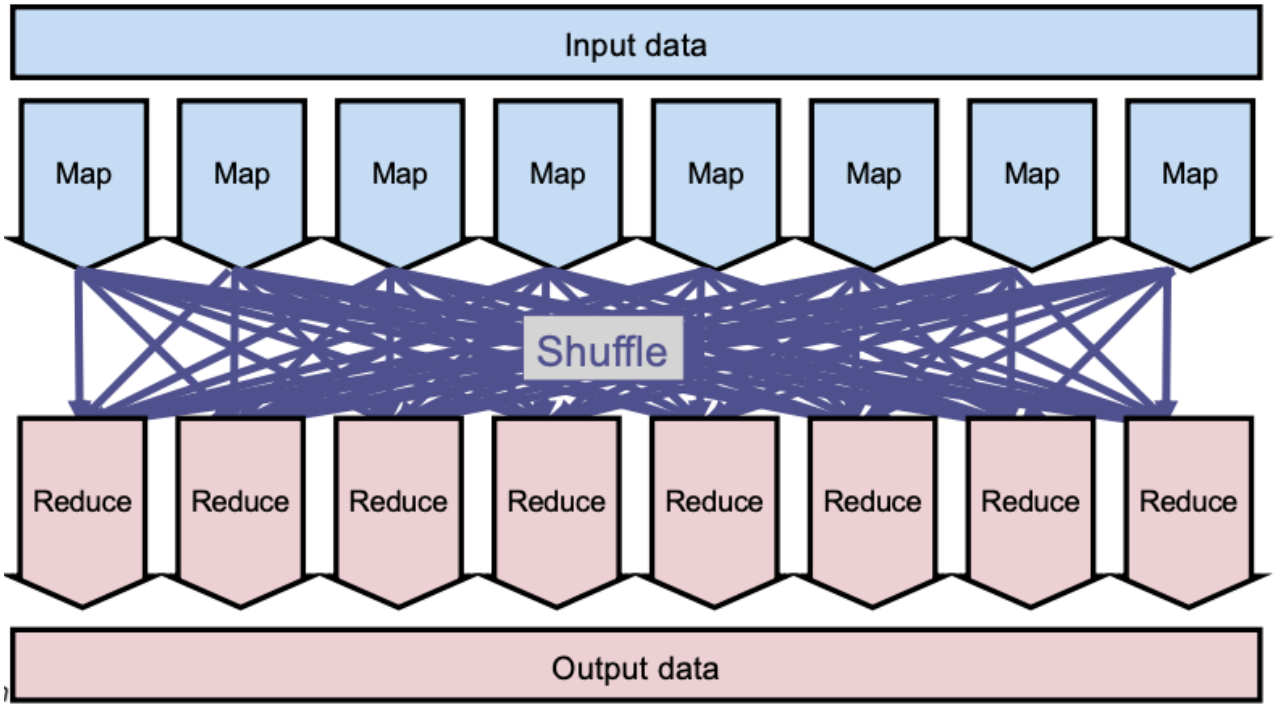
\includegraphics[width=0.6\textwidth]{Figures/StandardMapReduce.png}
    \caption{Standard Map Reduce}\label{fig:StdMapRed}
\end{figure}

\subsection{The MapReduce Model}

\subsubsection{Key-Value Pairs}
In MapReduce, the input data, intermediate data, and output data are all made of a large collection of key-value pairs (with the keys not necessarily unique, and not necessarily sorted by key). The types of the keys and values are known at compile-time (statically), and they do not need to be the same across all three collections. In practice, however, it is quite common that the type of the intermediate key-value pairs is the same as that of the output key-value pairs.

\subsubsection{Logical Walkthrough}
Everything starts with partitioning the input. MapReduce calls the partitions “splits”. Each key-value will be fed into a map function, mapping each value to a new intermediary key (e.g. from Key 1 of the input layer to Key \uproman{1} in the intermediate layer). However, as you can imagine, it would be extremely inefficient to do it pair by pair, thus, the map function is called in batches, on each split. Next, the new key-value pairs can be put together logically and logically sorted by their keys. Now, partition the table again, making sure the pairs with the same key are always in the same partition (but the partition can have pairs with several keys). The reduce function must then be called, for every unique key, on all the pairs with that key, outputting zero, one or more output pairs (in most cases it is one, and the key in the output layer is usually also the same as in the intermediate layer). Just like the map function, the reduce function is called in batches, on each intermediate partition (multiple calls, one per unique key). See \cref{fig:OverallMapRed} for a visual overview of the logical walkthrough of MapReduce.

\begin{figure}[h]
    \centering
    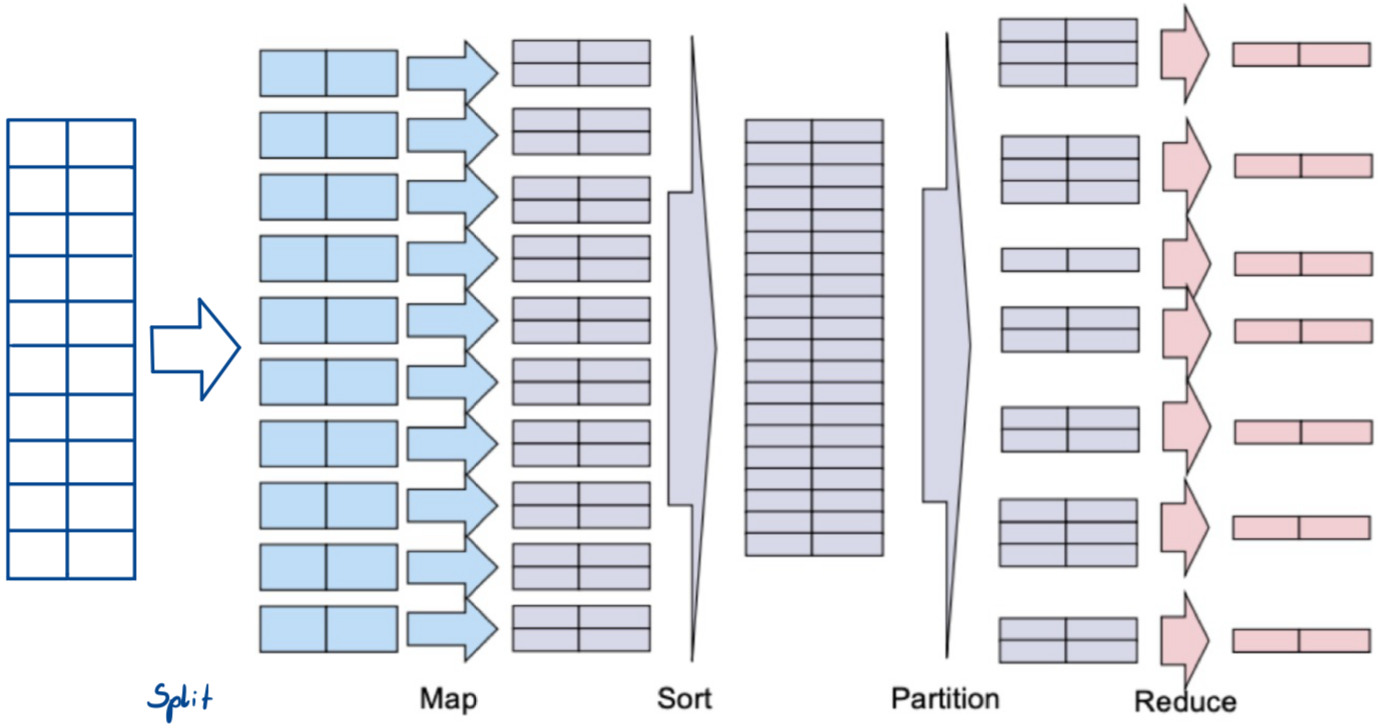
\includegraphics[width=0.9\textwidth]{Figures/OverallMapReduce.png}
    \caption{Overall MapReduce}\label{fig:OverallMapRed}
\end{figure}

\subsection{MapReduce Architecture}
MapReduce can read its input from many places as we saw: a cloud storage service, HDFS, a wide column store, etc. The data can be Petabyte-sized, with thousands of machines involved.

On a cluster, the architecture is centralized, just like for HDFS and HBase. In the original version of MapReduce, the main node is called JobTracker, and the worker nodes are called TaskTrackers. In fact, the JobTracker typically runs on the same machine as the NameNode (and HMaster) and the TaskTrackers on the same machines as the DataNodes (and RegionServers). This is called “bring the query to the data.” If using HDFS, then most of the time, for the map phase, things will be orchestrated in such a way that there is a replica of the block corresponding to the split on the same machine (since it is also a DataNode...), meaning that it is a local read and not a network connection.

As the map phase progresses, there is a risk that the memory becomes full. But we have seen this before with HBase: the intermediate pairs on that machine are then sorted by key and flushed to the disk to a Sequence File. And as more flushes happen, these Sequence Files can be compacted to less of them, very similarly to HBase’s Log-Structured Merge Trees.

When the map phase is over, each TaskTracker runs an HTTP server listening for connections, so that they can connect to each other and ship the intermediate data over to create the intermediate partitions ensuring that the same keys are on the same machines. This is the phase called shuffling. Then, the reduce phase can start.

Note that shuffling can start before the map phase is over, but the reduce phase can only start after the map phase is over.

When the reduce phase is completed, each output partition will be output to a shard (as we saw, a file named incrementally) in the output destination (HDFS, S3, etc) and in the desired format.

\subsection{MapReduce Input and Output Formats}

\subsubsection{Impedance Mismatch}

As the reader will have noticed, MapReduce only reads and writes lists of key-value pairs, where keys may be duplicates and need not appear in order. However, the inputs we considered are not key-value pairs. So we need an additional mechanism that allows MapReduce to interpret this input as key-value pairs.

For tables, whereas relational or in a wide column stores, this is relatively easy: indeed, tables have primary keys, consisting of either a single column or multiple columns. Thus, each tuple can be interpreted as a key-value pair, where the key is the (sub)tuple containing all the values associated with columns that are part of the primary key, while the value is the (sub)tuple containing the values associated with all other columns.

A key-value-pair is then one row of the tabel. The first column corresponds to the key and the remaining columns to the values.

\subsubsection{Mapping Files to Pairs}

How do we read a (possibly huge) text file as a list of key-value pairs? The most natural way to do so is to turn each line of text in a key value pair: the value is the string corresponding to the entire line, while the key is an integer that expresses the position (as a number of characters), or offset, at which the line starts in the current file being read. A small variation consists in reading N lines at a time, mapping them to a single key-value. Another variation consists of treating a character (picked by the user) specially, as the separator between the key and the value (e.g. space, semicolon, etc.).


\subsection{Examples}

\subsubsection{Counting Words}

We can count the words within each line similar to our motivation example with the cats, by mapping each line key-value to several key-values, one per word and with a count of 1. This gives us our map function. The reduce function is then obtained by summing the values with the same key, and keeping the same key. The output will then consist of a list of unique key-values, with one key for each word, and the number of its occurrences as the associated value.

\subsubsection{Selecting}

Filtering the lines containint a specific word can easily be done by having a map function that outputs a subset of its input, based on some predicate provided by the user. Here we notice that the output of the map phase already gives us the desired result; we still need to provide a reduce function, which is taken trivially as the identity function. This is not unusual.

In fact, what we have just implemented in MapReduce is nothing else than a selection operator from the relational algebra.

\subsubsection{Projecting}

What about projection on some input in the JSON Lines format? MapReduce doesn’t know anything about attributes. So it is up to the user to parse, in their code, each line to a JSON object (e.g., if using Python, to a dict). Then, the map function can project this object to an object with less attributes. Then, the map function can project this object to an object with less attributes. MapReduce will then output the results as one or several output files in the JSON Lines format.

\subsection{Combine Functions and Optimization}

In our counting example, we created an intermediate key-value for each occurrence of a word with a value set to 1. But what if a word appears 5 times on the same line? In this case, we can replace the corresponding key-value pairs with just one pair, with the value 5. Doing so is called combining and happens during the map phase.

Thus, in addition to the map function and the reduce function, the user can supply a combine function. This combine function can then be called by the system during the map phase as many times as it sees fit to “compress” the intermediate key-value pairs. Strategically, the combine function is likely to be called at every flush of key-value pairs to a Sequence File on disk, and at every compaction of several Sequence Files into one.

However, there is no guarantee that the combine function will be called at all, and there is also no guarantee on how many times it will be called. Thus, if the user provides a combine function, it is important that they think carefully about a combine function that does not affect the correctness of the output data. In fact, in most of the cases, the combine function will be identical to the reduce function, which is generally possible if the intermediate key-value pairs have the same type as the output key-value pairs, and the reduce function is both associative and commutative. This is the case for summing or multiplying values2 as well as for taking the maximum or the minimum, but not for an unweighted average. As a reminder, associativity means that $(a + b) + c = a + (b + c)$ and commutativity means that $a + b = b + a$.


\subsection{MapReduce Programming API}

In Java, the user needs to define a so-called Mapper class that contains the map function, and a Reducer class that contains the reduce function.

\subsubsection{Mapper Classes}
A map function takes in particular a key and a value. Note that it outputs key-value pairs via the call of the write method on the context, rather than with a return statement. That way, it can output zero, one or more key-values. A Mapper class looks like so:

\begin{lstlisting}[style=Java]
import org.apache.hadoop.mapreduce.Mapper;
public class MyOwnMapper extends Mapper<K1, V1, K2, V2>{
  public void map(K1 key, V1 value, Context context)
        throws IOException, InterruptedException
    {
        ...
        K2 new-key = ...
        V2 new-value = ... context.write(new-key, new-value); ...
    }
}
\end{lstlisting}

\subsubsection{Reducer Classes}

A reduce function takes in particular a key and a list of values. Note that it outputs key-value pairs via the call of the write method on the context, rather than with a return statement. That way, it can output zero, one or more key-values. A Reducer class looks like so:

\begin{lstlisting}[style=Java]
import org.apache.hadoop.mapreduce.Reducer;
public class MyOwnReducer extends Reducer<K2, V2, K3, V3> {
public void reduce (
        K2 key,
        Iterable<V2> values,
        Context context)
    throws IOException, InterruptedException
    {
        ...
        K3 new-key = ...
        V3 new-value = ... context.write(new-key, new-value); ...
    }
}
\end{lstlisting}

\subsection{Using Correct Terminology}

Let us now have a word of warning: the terminology “Mapper” and “Reducer” should only be used in the context of naming classes and files, but never when describing the MapReduce architecture. Even less so with “Combiner.”

\subsubsection{Functions}

\begin{itemize}
    \item A map function is a mathematical, or programmed, function that takes one input key-value pair and returns zero, one or more intermediate key-value pairs.
    \item A reduce function is a mathematical, or programmed, function that takes one or more intermediate key-value pairs (with the same key) and returns zero, one or more output key-value pairs.
    \item A combine function is a mathematical, or programmed, function that takes one or more intermediate key-value pairs (with the same key) and returns zero, one or more intermediate key-value pairs.
\end{itemize}

\subsubsection{Tasks}

\begin{itemize}
    \item Then, a map task is an assignment that consists in a (sequential) series of calls of the map function on a subset of the input. There is one map task for every input split, so that there are as many map tasks as partitions of the input.
    \item A reduce task is an assignment that consists in a (sequential) series of calls of the reduce function on a subset of the intermediate input. There are as many reduce tasks as partitions of the list of intermediate key-value pairs.
\end{itemize}

We insist that the calls within a task are sequential, meaning that there is no parallelism at all within a task. You can think of it as a for loop calling the function repeatedly, with the size of the for loop being, in a typical setting, between 1,000 and 1,000,000 calls.

There is no such thing as a combine task. Calls of the combine function are not planned as a task, but is called ad-hoc during flushing and compaction.

\subsubsection{Slots}

The map tasks are processed thanks to compute and memory resources (CPU and RAM). These resources are called map slots. One map slot corresponds to one CPU core and some allocated memory. The number of map slots is limited by the number of available cores. Each map slot then processes one map task at a time, sequentially. This means that the same map slot can process several map tasks.

The resources used to process reduce tasks are called reduce slots. Again, one reduce slot corresponds to one CPU core and some allocated memory. The number of reduce slots is limited by the number of available cores. Each reduce slot then processes one reduce task at a time, sequentially. This means that the same reduce slot can process multiple reduce tasks.

So, there is no parallelism either within one map slot, or one reduce slot. In fact, parallelism happens across several slots. In a typical MapReduce job, there will be more tasks than slots. Initially, each slot will receive one task, and the other tasks are kept pending. Every time a slot is done processing a task, it receives a new task from the pending list, and so on, until no task is left: then, some slots will remain idle until all tasks have been processed. If a task fails, it can be reassigned to another slot.

\subsubsection{Phases}

The map phase thus consists of several map slots processing map tasks in parallel and the reduce phase consists of several reduce slots processing reduce tasks in parallel. This is a summary of how functions, tasks, slots and phases fit together and within cluster nodes:

\begin{figure}[h]
    \centering
    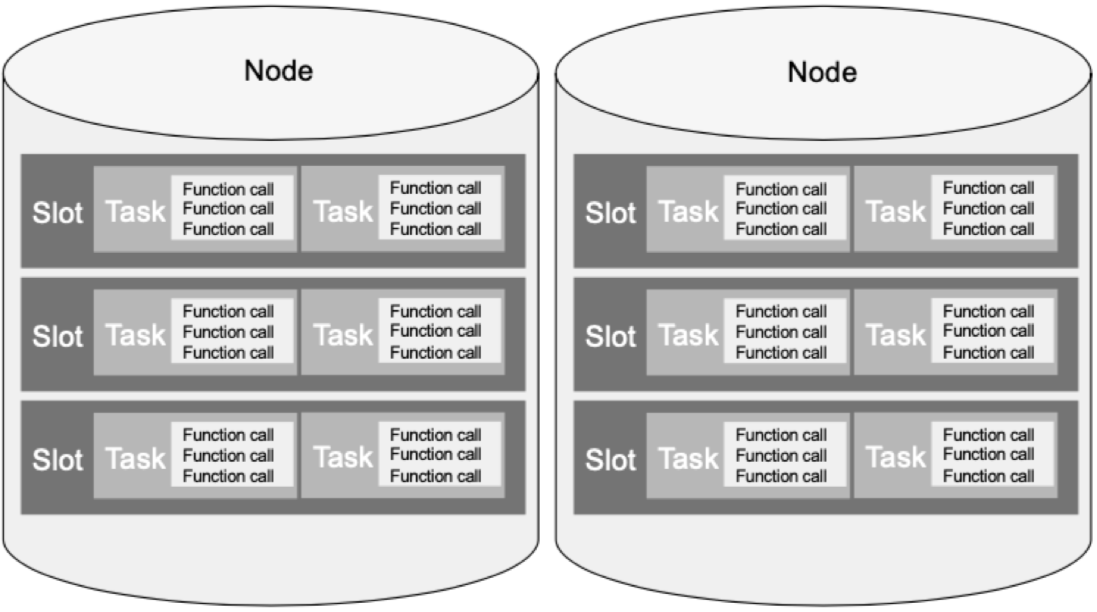
\includegraphics[width=0.7\textwidth]{Figures/MapReduceNodes.png}
    \caption{Summary of how functions, tasks and phases fit together and within cluster nodes.}
\end{figure}

\subsection{Impedance Mismatch: Blocks vs. Splits}
HDFS blocks have a size of (at most) 128 MB. In every file, all blocks but the last one have a size of exactly 128 MB. Splits, however, only contain full records: a key-value pair will only belong to one split (and thus be processed by one map task). This means that, while most key-value pairs will be in the same block, the first and/or last key-value pair in a split will be spread across two blocks. This means that, while most of the data is obtained locally, getting the first and/or last record in full will require a remote read over the HDFS protocol. This, in turn, is also the reason why the HDFS API gives the ability to only read a block partially.